% About Unity

\section{External resources}
The Design Review application was implemented by using several pre-made assets.
When the application is started user is positioned into a oiltank model, which was provided by DNV GL. 
This model is of high fidelity and was originally developed for the DNV GL Survey Simulator, an application to train surveyors.

\begin{figure}%[h!] %[H]
	\frame{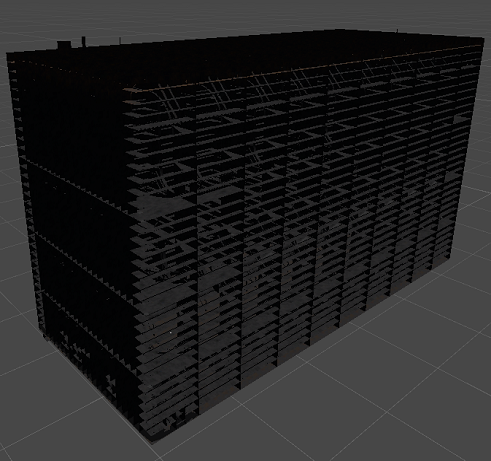
\includegraphics[width=0.5\linewidth]{pictures/tank/back.png}}
	\frame{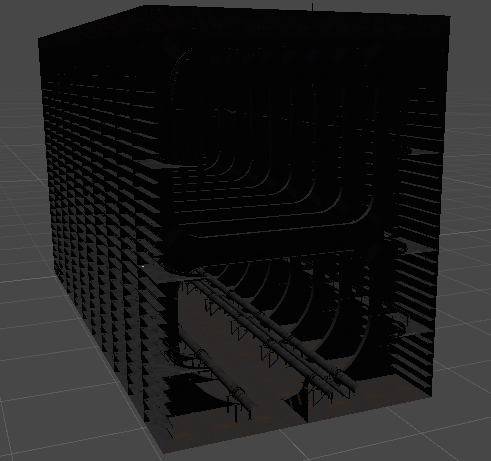
\includegraphics[width=0.5\linewidth]{pictures/tank/half_profile.png}}
	\caption[The Oil tank model]{The Oil tank model from the outside}
	\label{fig:tank_outside}
\end{figure} 

The application also makes use of several "best practice" assets from Leap Motion, Oculus VR and SteamVR to ensure that these devices function
as optimally as possible. From Leap Motion the \texttt{LeapHandController} is utilized, which is a prefab (gameObject), with several important scripts attached to
it. Leap motion provided hand models are also being used, which was provided from the Leap Motion Hands-module. More specifically 
the \texttt{RiggedPepperCutHands} were used, but any other of the hand models could be used as easily.

From Oculus VR two prefabs is used. The first is \texttt{OVRCameraRig}, which is the recommended camera setup for using the Oculus Rift HMD. This 
prefab sets several important settings to ensure that both the head tracking and visual performance is as optimal as possible. The 
second prefab which is used is one called the \texttt{GazePointerRing}. This was showcased in a demo unity implementation by OculusVR
and is essentially a cursor that exist in the game world a fixed length in front of the user. As regular crosshair (which are drawn directly on the screen space)
isn't allowed in VR (more about this later), the \texttt{GazePointerRing} serves as a crosshair. 
From SteamVR the \texttt{[CameraRig]} prefab is used, which essentially does the same configurations as the \texttt{OVRCameraRig} does, but with the HTC Vive HMDs in mind.

The Design review application also makes use of Hover UI Kit, an open source project for creating VR/AR-enabled, customizable and dynamic user interfaces. 
This kit was vital in rapidly prototyping a gesture-enabled menu and a virtual keyboard to the annotation forms.

\section{The architecture}
\begin{figure}%[h!] %[H]
	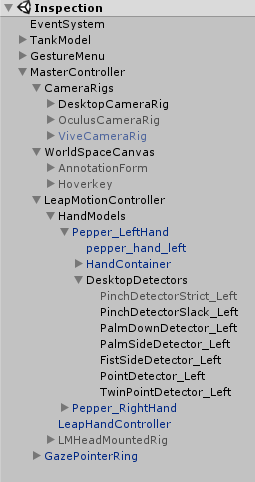
\includegraphics{pictures/unity_hierarchy.png}
	\caption[The Unity project hierarchy of the Design Review Application]{The Unity project hierarchy of the Design Review Application}
	\label{fig:unity_hierarchy}
\end{figure} 

The Unity project has four top-level game objects, as visible in \ref{fig:unity_hierarchy}. 
These will be covered by their own sections, with subsections detailing their important child game objects where appropriate.

% In short terms EventSystem is responsible for processing and handling events and input actions in the scene.
% The TankModel game object contains several child objects that together make up the oiltank-model.
% GestureMenu contains the menu, all its interactable buttons and several scripts.
% The MasterController . 

\section{The master controller}
The \texttt{MasterController} game object represents the player model and contains many of the most important game objects, in addition to
holding many key scripts. The \texttt{MasterController}'s transform, with its position, rotation and scale, represents the user's position and orientation, 
and every child object of \texttt{MasterController} will have a position, rotation and scale that is relative to its own. This ensures
that e.g.~the camera will always "follow" the user. Because this game object is so essential, we will cover several important components and
child objects in the following section.

\begin{figure}%[h!] %[H]
	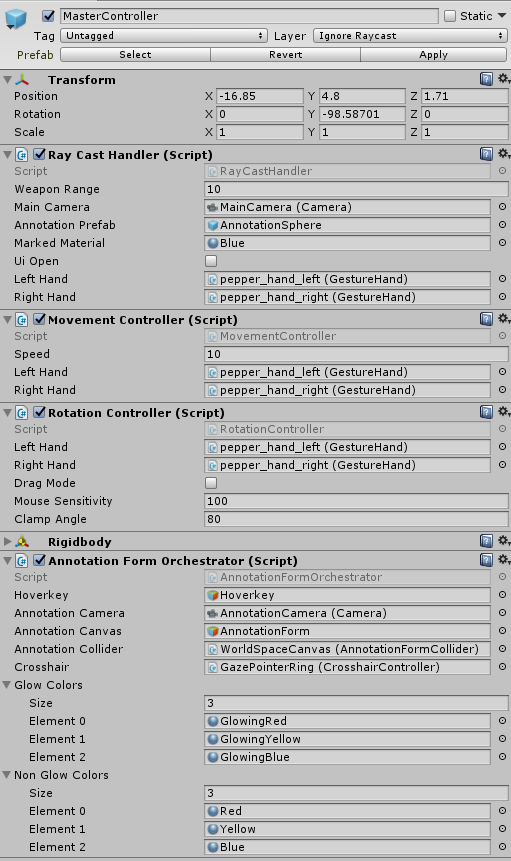
\includegraphics{pictures/unity_inspector.png}
	\caption[The \texttt{MasterController} components]{The \texttt{MasterController} components seen in the Unity Inspector view.}
	\label{fig:unity_inspector}
\end{figure} 

\subsection{The camera rigs}
The \texttt{CameraRigs} game objects holds three different game object, which each represents its own camera-setup: \texttt{DesktopCameraRig}, which is meant to be used
without virtual reality, \texttt{OculusCameraRig}, meant to be used with Oculus Rift HMDs, and \texttt{ViveCameraRigs}, meant to be used with the HTC Vive.
For the application to run successfully one of these rigs should be enabled, while the other two should be disabled.
This can be done by switching between the three rigs in the dropdown-menu named Rig, which is present on the \texttt{CameraRigs} game object itself and
implemented in the \texttt{CameraRigSetup} script. In addition to ensuring that only the correct rig is enabled, 
the \texttt{CameraRigSetup} script also does several other operations. One of these is ensuring that the field of view is set to 60 degrees if the desktop rig 
is selected, as this can wrongfully be set to a HMD's value if a HMD is connected to the computer. When a virtual reality rig is used the field of view is 
set automatically by the HMD software. Another thing done by the script is to decide wheter a two dimensional crosshair/cursor should be drawn on the screen space
(in case of the desktop rig), or if a three dimensional crosshair/cursor (i.e the \texttt{GazePointerRing}) should be drawn in the world space. 

\subsection{The world space canvas}
The \texttt{WorldSpaceCanvas} is a canvas object, which in Unity serves as a container for other user interface elements, such as buttons and input fields, 
and is rendered in world space. It is thus diegetic and exists there like other 3D objects.

In applications that don't utilize virtual reality, canvases and other UI elements are usually non-diegetic (i.e they don't exist within the game world), 
and in 2D and drawn directly to the screen space (as opposed to world space) using x- and y-coordinates.
With this approach one can specify e.g.~a position by its x- and y-coordinate, where \{0, 0\} usually represents the top-left of the display.
This changes in virtual reality applications, as the user's eyes are unable to focus on the screen space. An analogy to this would be to 
ask the user to read a letter while holding it 2-3 centimeters from their eyes. Because of this, elements appearing on the screen space is not rendered
in unity while running it with the virtual reality SDKs. 

\begin{figure}%[h!] %[H]
	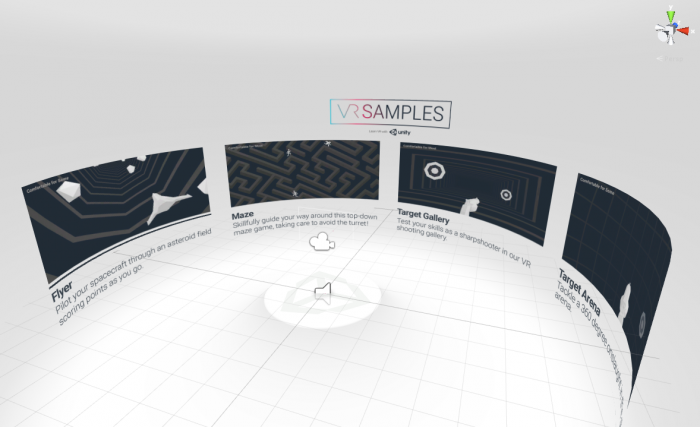
\includegraphics[width=\linewidth]{pictures/unity_vr_menu.png}
	\caption[An example of world-space (diegetic) user interfaces]{An example of world-space (diegetic) user interfaces~\citep{Unity}.}
	\label{fig:unity_vr_menu}
\end{figure} 

Another reason why the canvas is rendered in world space, and also the reason why this is the case in desktop mode, is because of our touch interaction.
To enable the user to click on buttons using his or her hands, the user interface must also exist in world-space so a collision can occur between the desired 
button and the hand models (that mimic the users hand). 

\texttt{WorldSpaceCanvas} is thus rendered in the world space, and is always positioned 0.8 unity meters (i.e the virtual representation of a meter in unity) 
in front of the user. The game object is thus always in the center of the camera, but is only visible and enabled when the user is editing an annotation. 
One issue with this approach is "clipping", i.e that the annotation form visually collides with another object (e.g.~the tank model or an annotation sphere) thus
obstructing it from view. To combat this \texttt{WorldSpaceCanvas} has a box-shaped collider component, which covers the canvas as well as the area between the canvas and the camera, 
and a script called \texttt{CanvasCollider}, which keeps track of objects that's within the collider component. When the user wish to edit an annotation, and the 
\texttt{AnnotationForm} and \texttt{Hoverkey} becomes active, the objects within the canvas' collider is disabled, thus hiding objects that could potentially
obstruct the whole, or parts of, the canvas. The objects are enabled again once the users is done editing the annotation (i.e when the user clicks "submit", "cancel" or "delete").

\begin{figure}%[h!] %[H]
	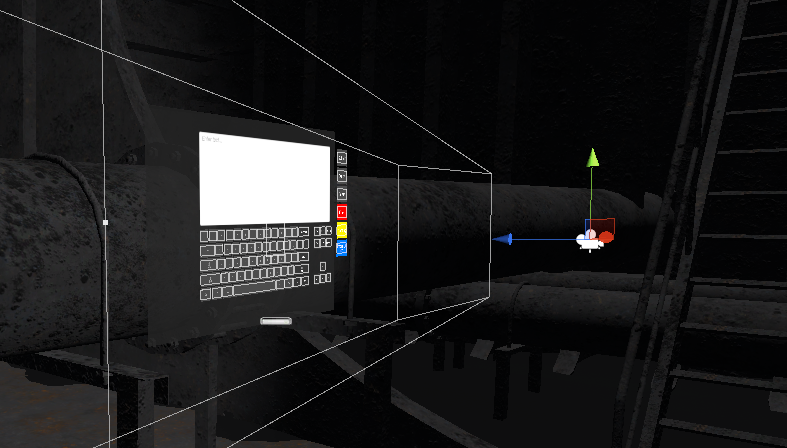
\includegraphics[width=\linewidth]{pictures/tank/worldspacecanvas_scene.png}
	\caption[The \texttt{WorldSpaceCanvas} as seen in the Unity Scene View]{The \texttt{WorldSpaceCanvas} as seen in the Unity Scene View.}
	\label{fig:worldspacecanvas_scene}
\end{figure} 

\begin{figure}%[h!] %[H]
	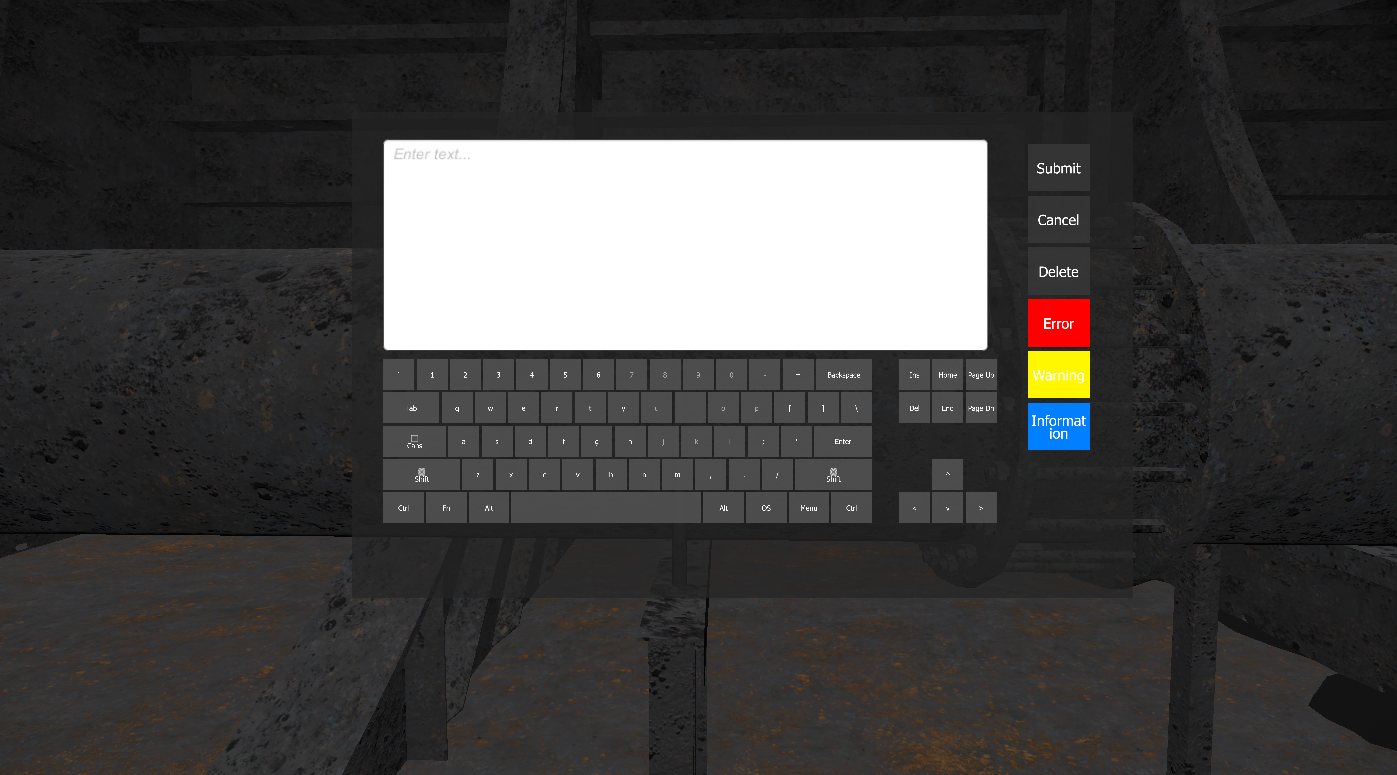
\includegraphics[width=\linewidth]{pictures/tank/worldspacecanvas_ingame.png}
	\caption[The \texttt{WorldSpaceCanvas} as seen in the Unity Game View]{The \texttt{WorldSpaceCanvas} as seen in the Unity Game View.}
	\label{fig:worldspacecanvas_ingame}
\end{figure} 

The \texttt{WorldSpaceCanvas} has two child game objects: \texttt{AnnotationForm} and \texttt{Hoverkey}. 
\texttt{AnnotationForm} currently only contains a inputfield-object and a background rectangle, but can in future iteration grow to 
contain other user interaction elements. The \texttt{Hoverkey} game object represents the touch keyboard and is part of the HoverUI-kit.
In addition to the keyboard six other similar buttons are also present: Submit, Cancel, Delete, Error, Warning and Information (see \ref{fig:worldspacecanvas_ingame}).

\subsection{The Leap Motion Controller}
The \texttt{LeapMotionController} game object contains objects related to the Leap Motion device and gesture recognition and consist primarily of the hand models, necessary 
scrips and detectors. In the game object \texttt{HandModels} there is one object-representation of the left hand, called \texttt{Pepper\_LeftHand}, and one for the 
right hand, called \texttt{Pepper\_RightHand}. These objects have their own hand models (as there needs to be different models for the left and right hand) and their 
own detector objects (as a detector can/should only observe one hand). Each "hand" thus have its own list of detectors called \texttt{Detectors}. 
These are the definition and implementation of the gesture scheme that were discussed in \ref{sec:gesture_design}. In addition to detectors, each
hand also have its own instance of the \texttt{GestureHand} class, which is an important component to keep track of hand states and resources, and
it exposes utility function to other classes. 

\subsection{The GestureHand class}
The \texttt{GestureHand} class is assigned as a component to each hand object, and contain several important variables.
\begin{itemize}
	\item \texttt{bool isLeftHand} - Keeps track of whether this instance belong to the left or the right hand.
	\item \texttt{GameObject handModel} - A reference to the unity game-object that contains the handModel this gesturehand instance is relevant for.
	\item \texttt{Material[] handMaterials} - An array of different material for the hand model. These are swapped between when e.g.~a certain gesture is brecognized and tracked.
	\item \texttt{GestureHand otherHand} - A reference to the other GestureHand-instance. For the lefthand GestureHand-instance this variable thus point to the right hand GestureHand
			hand-instance.
	\item \texttt{GameObject detectors} - A reference to the gameobject that hold/is parent of this hands detectors.
	\item \texttt{bool combineGestures} - Keeps track of whether the user is using a combined XYZ axis gesture scheme or if these movement gesture are kept separate (see \ref{sec:combined-movement}).
	\item \texttt{Vector gestureOriginPosition} - Holds the x-, y- and z- coordinates of the palm when the current gesture was recognized.
	\item \texttt{HandState handState} - Holds one of several HandState enum values that represent the hand state. This variable has one of the following enum values:
			NONE = 0, PINCH = 1, PALM\_DOWN = 2, PALM\_SIDE = 3, FIST = 4, SINGLE\_POINT = 5, DOUBLE\_POINT = 6 or DISABLED = 7 (see \ref{tab:handstates}).  
\end{itemize}

% \begin{table}[]
% \centering
% \caption{The instance variables of the \texttt{GestureHand} class}
% \label{my-label}
% \begin{tabular}{p{2cm}| p{2cm} | p{4cm}}
% 	\textbf{Data type} &  \textbf{Variable name} &   \textbf{Description} \\
% 	bool & isLeftHand &   Keeps track of whether this instance belong to the left or the right hand. \\
% 	GameObject & handModel & A reference to the unity game-object that contains the handModel this gesturehand instance is relevant for.  \\
% 	Material[] & handMaterials & An array of different material for the hand model. These are swapped between when e.g.~a certain gesture is brecognized and tracked.  \\
% 	GestureHand & otherHand & A reference to the other GestureHand-instance. For the lefthand GestureHand-instance this variable thus point to the right hand GestureHand hand-instance.  \\
% 	GameObject & detectors & A reference to the gameobject that hold/is parent of this hands detectors.  \\
% 	bool &  combineGestures & Keeps track of whether the user is using a combined XYZ axis gesture scheme or if these movement gesture are kept separate (see \ref{sec:combined-movement}).  \\
% 	Vector & gestureOriginPosition & Holds the x-, y- and z- coordinates of the palm when the current gesture was recognized.  \\
% 	HandState & handState & Holds one of several HandState enum values that represent the hand state. This variable has one of the following enum values:
% 			NONE = 0, PINCH = 1, PALM\_DOWN = 2, PALM\_SIDE = 3, FIST = 4, SINGLE\_POINT = 5, DOUBLE\_POINT = 6 or DISABLED = 7.  
% \end{tabular}
% \end{table}

\begin{table}[]
\centering
\label{tab:handstates}
\begin{tabular}{p{1cm}| p{3.5cm} | p{6cm}}
	\textbf{ID} &  \textbf{Variable name} &   \textbf{Implication} \\\\
	0 & NONE & No gesture is being performed. \\\\
	1 & PINCH & User can rotate by the y- and z-axis \\\\
	2 & PALM\_DOWN & User can move along the y-axis.  \\\\
	3 & PALM\_SIDE & User can move along the x-axis.  \\\\
	4 & FIST & User can move along the z-axis.  \\\\
	5 & SINGLE\_POINT & User is placing/has placed point-annotation.  \\
	6 & DOUBLE\_POINT & User is placing/has placed object-annotation.  \\
	7 & DISABLED & The detectors are disabled and no gesture and hand state can be achieved before enabling them.  
\end{tabular}
\caption{The\texttt{GestureHand} class' hand states}
\end{table}

The \texttt{GestureHand} class also contains several important functions that are called when a certain gesture is activated or deactivated.
\texttt{void ActivateGesture(int gestureCode)} is called by a detector when it becomes active, i.e when its criteria are met and the gesture it represent is recognized.
It then signals the \texttt{GestureHand} class with its code/signature so \texttt{GestureHand} knows which detectors called it.
If a pinch gesture is detected by the left hand pinch detector the left hand \texttt{GestureHand} class' \texttt{ActivateGesture} is thus called with the argument "1".
From a design standpoint one should be able to send the Handstate.PINCH enum as a value, but then this function wouldnt be exposed in the Unity Inspector interface (which
only seem to accept primitive or built-in argument types). 

Once this function is called it sets the hand state to the value of the gestureCode, sets the gesture origin position and switches the hand materials.
Hand material switches is done by assigning the material at index \texttt{gestureCode} in the \texttt{handMaterials} list to the hand model, so 
if a pinch gesture is a performed the hand model is assigned the material at \texttt{handMaterials[1]}. The HandState enums and the hand material list thus 
follow the same sorting order. 

The \texttt{GestureHand} class also has the function \texttt{void DeactivateGesture()}, which is called by a detector when it becomes deactivated. 
This function simply resets the hand state by setting it to HandState.NONE (NONE = 0) and assign the material at \texttt{handMaterials[(int) HandState.NONE]} (i.e 0) to the
handmodel. \texttt{GestureHand} also contains the functions \texttt{enableDetectors()} and \texttt{disableDetectors()}, which 
enables or disables all the detectors that belongs to the same hand as the current \texttt{GestureHand} instance. These are used in two scenarios:
When the user switches between having gestures enabled and disable by using the menu options "Enable Gestures" and "Disable Gestures" and when an annotation 
is edited. When an annotation is edited, and the annotation form is open, gestures that one can use otherwise (e.g~the movement and rotation gestures) are disabled.

 
\subsection{The detectors}
The detectors are represented as game objects and children of the \texttt{Detectors} game object under each hand game object. 
Each of these detector objects have the naming convention <gesture name> + "Detector" + <optional specifier> + "\_" + <handedness: Left or Right>, 
e.g.~\texttt{PinchDetectorStrict\_Left} and \texttt{FistDetector\_Right}. A certain detector of one hand is usual identical to the equivalent detector for the 
other hand with a few exception. These differences between hands are usually minor and will be mentioned when applicable. The detectors used in this implementation
utilizes a combination of several Leap Motion provided detectors, as these both cover the functional needs and are considered best practice. 
The Leap Motion provided detectors can as such be regarded as "base detectors", while the detectors that represents gestures in this implementation
can be regarded as "composite detectors". To differentiate between these two categories, the base detectors will be written in \textit{italic} or plain text, while
the composite detectors and game objects will be written in \texttt{monospace}.
The Leap Motion provided detectors utilized in the implementation is \textit{DetectorLogicGate}, \textit{PinchDetector}, \textit{ExtendedFingerDetector}, 
\textit{PalmDirectionDetector} and \textit{FingerDirectionDetector}.

The Leap motion base detectors provides some important parameters that can be set on a per detector instance basis, which often relates to thresholds values (e.g.~on/off values) and discrete
values (e.g~extended or not extended). Finding the optimal values for a certain gesture can often be the subject of a lot of adjustment and tweaking, as vision-based gesture recognition
technology often or always will be someone unprecice compared to e.g.~mouse and keyboard. The challenge is thus to find values that give a high amout of true positives (e.g.~the user attemps a gesture
and the gesture was recognized) and a low amount of false positives (e.g.~the user did not attempt a gesture and a gesture was recognized). 
During the implementation phase these values were adjusted several times in pursuit of the optimal values, and during the evaluation phase this was a much discussed topic were users often 
has their own "gesture sensitivity preferences" (this will be review in the next chapter). First the gesture implementations will be reviewed. 


\subsubsection{The PinchDetectorStrict and PinchDetectorSlack}
The \texttt{PinchDetectorStrict} and \texttt{PinchDetectorSlack} were originally one detector called \texttt{PinchDetector}, but was split up to represent two 
different options for the user. Both detectors utilize the base \textit{PinchDetector} script provided by the Leap Motion detection utilities, while the strict version
also uses the \textit{ExtendedFingerDetector}. The \texttt{PinchDetector} measures the distance between the tip of the thumb and index finger, and if these are below
a certain threshold (i.e the activate distance) the detector is active and signals \texttt{gestureCode}. If the distance grow larger than a set deactivate distance
the detector is deactivated. The activate distance used is 0.03 meter, while the deactivate distance is 0.06 meter. 

One problem with only having distance between the two finger tips as a criterion for the pinch gesture is that there would sometimes be false positives 
(i.e unintentional pinch gestures could occur). This was especially the case when attemping to perform the fist gesture as the distance between the tip of the
thumb and index finger is relatively small when the hand is a fist, and the application could thus sometimes perform a pinch gesture instead of a fist gesture.
Because of this the stricter version \texttt{PinchDetectorStrict} was created. This uses the same criterion as \texttt{PinchDetectorSlack}, but it also requires
that at least two fingers are extended. This is accompished by using the \textit{ExtendedFingerDetector} and \textit{DetectorLogicGate}. 
The finger states of the \textit{ExtendedFingerDetector} for all individual fingers are set to "either", meaning that, individually, each finger can 
be either extended or not extended, but on the "minimum extended" parameter 2 is set, while "maximum extended" is set to 5, 
meaning that anything between two and five fingers can be extended. 

\subsubsection{The PalmDownDetector}
The \texttt{PalmDownDetector} uses a PalmDirection detector and an ExtendedFinger detector, which is AND'ed by a DetectorLogicGate. 
The PalmDirectionDetector is configured to become active when the palm is pointing within 30 degrees of {0, -1, 0} (x = 0, y = -1, z = 0) direction, relative to the camera.
The coordinate system used functions just as if the three-dimensional axis had been drawn on the screen, so e.g.~ the coordinates {0, 0, 1} would be directly forward, while
{1, 0, 0} would be to the right.

The coordinates used for the PalmDirection Detector thus means that from the perspective of the camera, the palm should face directly downwords such that the 
palms are as parallell to the ground or table top.
The PalmDirectionDetector is also configured with an "On Angel" of 30 degrees and an "Off Angle" of 50. The detector is thus activated as long as the palm points within 
30 degrees of the desired direction, and is deactivated if the palm directions surpasses the threshold of 50 degree from the {0, -1, 0} direction.

The \texttt{PalmDownDetector} also used an ExtendedFingerdetector, as was covered in the previous section. This one is configured to require that 
the index-, middle, ring and pinky finger have to be extended, which the thumb can be either. 

\subsubsection{The PalmSideDetector}
The \texttt{PalmSideDetector} is quite similar to the \texttt{PalmDownDetector} and uses the same detectors, but with a different configuration. 
Although the settings used for the DetectorLogicGate and the ExtendedFingerDetector are very similar, the settings for the PalmDirectionDetector differs.
Unlike the \texttt{PalmDownDetector}, where both hands are required to point in the direction {0, -1, 0} to perform the gesture, the \texttt{PalmSideDetector} makes 
a distinction here. This is because requiring the palm direction {1, 0, 0} (right) is reasonable for the left hand, as it is within its natural range of motion, but
for the right hand this requires the whole arm to twist. The required palm direction for the left hand is thus {1, 0, 0} (right), and {-1, 0, 0} (left) for the right hand, both
with an "On Angel" of 30 degrees and an "Off Angle" of 50.

\subsubsection{The FistDetector}
The \texttt{FistDetector} is prehaps the simplest of the detectors and only uses the ExtendedFingerDetector.
The ExtendedFingerDetector is simply configured to require that no finger is extended. 
As such the minimum- and maximum amount of fingers extended are both set to 0, and all finger have their required state set to "Not Extended"

\subsubsection{The SinglePointDetector}
The \texttt{SinglePointDetector} uses two detectors, ExtendedFingerDetector and FingerDirectionDetector, bound together with an AND-DetectorLogicGate.
The ExtendedFingerDetector here requires that the index finger is extended and that the middle-, ring- and pinky fingers are not extended (both thumb states are accepted).
The FingerDirectionDetector is set to be active when the index finger points within 15 degrees of the direction {0, 0, 1}, relative to the camera.
Both the "On Angle" and "Off Angle" settings are set to 15 in this detector, as, unlike the previously mentioned detectors, this one is not of a "continous nature".
Simply put, the previous gestures can last as long as the gesture is held, and while this is the case the application continously watches the active hands and responds to
hand movements. The single- and double point detectors are techniqually also continous and can last as long as the user desires, 
but as soon as these gestures are activated their discrete action is performed. After this action has been performed no other action will be performed by the same
and while the same gesture is kept. In the case of both the single- and double point detectors,an annotation is either placed or edited upon activation. 
If a user thus with to place an annotation and immediatly edit it, he or she has to use the approprate gesture, release the gesture and do the same gesture again.

\subsubsection{The DoublePointDetector}
The \texttt{DoublePointDetector} is similar to the \texttt{SinglePointDetector} and uses the same base detectors. 
The only implementational difference between this two is that the ExtendedFingerDetector is configured to require that both the index- and middle finger are extended, while
the ring- and pinky finger are contracted (both thumb states are accepted).












% Important child objects of MasterController include CameraRigs, which holds seperate camera rigs for either destop, oculus rift or htc vive usage, 
% WorldSpaceCanvas for drawing user interfaces in the game world, LeapMotionController for aspects related to the Leap Motion and
% GazePointerRing to enable the gazepointer ring when a virtual reality headset is used. These are all documented below.


